Um dos sistemas dinâmicos não lineares intrinsecamente instáveis mais estudados é o de pêndulo invertido, sendo comumente usado em \textit{benchmarks} para verificar a eficácia de métodos de controle. 

%Outro caso em que se é muito comum a implementação deste tipo de controlador é para o controle de estabilidade de um pêndulo invertido. Diversas são as abordagens que se encontram na literatura.
%Um pêndulo invertido é um sistema instável não linear comumente usado em \textit{benchmarks} para verificar a eficácia de métodos de controle. 
%A figura \autoref{fig:inverted-pendulum-diagram} ilustra o modelo de um pêndulo invertido. Este sistema é composto de uma barra rígida colocada verticalmente sobre um carro. O objetivo do sistema é manter a barra em equilíbrio oscilatório, fazendo com que ela não caia \cite{Arai2014}.
\iffalse
\begin{figure}[!htb]
    \centering
    \caption{Modelo de um pêndulo invertido}
    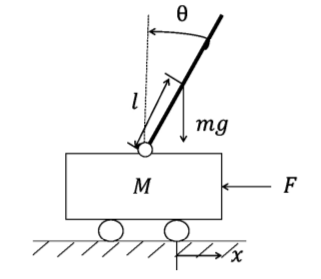
\includegraphics[width=0.4\textwidth]{./04-figuras/inverted-pendulum_diagram}
    \fonte{\cite[p.~416]{Arai2014}}
    \label{fig:inverted-pendulum-diagram}
\end{figure}

Na \autoref{fig:inverted-pendulum-diagram}, $M$ [$kg$] é a massa do carro, $m$ [$kg$] é a massa do pêndulo, $l$ [$m$] é metade do comprimento do pêndulo, $g$ [$m/s^2$] é a aceleração da gravidade e $\theta$ [$rad$] é o ângulo de desvio da barra em relação à posição vertical. O valor de cada variável de estado é calculada usando o método de Euller para um pequeno período de tempo $\tau$ [$s$].
\fi
\citeonline{Kim2000} compararam um controlador puramente LQR a um controlador híbrido, aliando o LQR a um controle neuro-fuzzy. A \autoref{fig:lqr-neuro-fuzzy-kim2000} mostra o esquema resultante. Neste modelo, a rede neural é configurada em paralelo ao controlador LQR. Este esquema consiste de um controlador LQR de ganho fixo que faz o sistema como um todo estável e um controlador realimentado que atualiza seus pesos internos para gerar o sinal de controle $u_{FN}$ contribuindo para a redução de tempo de convergência do sistema.

\begin{figure}[!htb]
    \centering
    \caption{Diagrama do controlador híbrido LQR-Neuro-Fuzzy implementado em \cite{Kim2000}}
    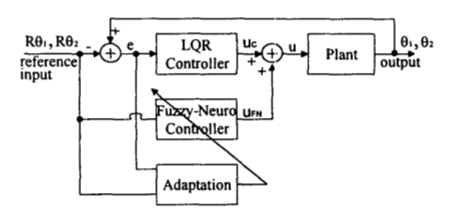
\includegraphics[width=0.6\textwidth]{./04-figuras/lqr_neuro_fuzzy_pendulum}
    \fonte{\cite[p.~416]{Kim2000}}
    \label{fig:lqr-neuro-fuzzy-kim2000}
\end{figure}

Resultados de simulação mostraram que o controlador híbrido LQR-Neuro-Fuzzy obteve menor erro na fase inicial de treinamento se comparado ao controlador LQR. Além disto, os resultados mostraram que o controlador proposto é mais eficiente que o LQR, obtendo melhor tempo de convergência.

\citeonline{Omatu1994} também propuseram um controlador híbrido aliando os controles LQR e Fuzzy. Neste caso, entretanto, os controladores operam em momentos diferentes. O controlador neuro-fuzzy atua sobre o sistema até que o pêndulo se aproxime da posição vertical. A partir de um ponto de referência, o controle passa a ser efetuado pelo controlador LQR. Neste caso, mais uma vez a inserção de um controle por neuro-fuzzy contribiu para a boa resposta do sistema.

Em \cite{Alata2001}, outro tipo de controlador híbrido LQR-Neuro-Fuzzy é proposto. Neste caso, os ganhos em diferentes regiões de operação são calculados usando o método LQR. Esses ganhos são tabulados com os estados correspondentes do ponto de operação. Então, um agrupamento subtrativo e o ANFIS são usados para contruir a base de dados e a base de regras do sistema de inferências fuzzy. Isto fornece um mecanismo suave de transição de um ponto de operação para outro. A eficácia da abordagem proposta foi provada por resultados experimentais de um pêndulo invertido.

Já \citeonline{Arai2014} utilizaram uma abordagem diferente, implementando um controlador puramente CVNF (\textit{Complex-Valued Neuro-Fuzzy}\footnote{Neuro-Fuzzy com Valores Complexos, tradução nossa}), que diz repeito a uma expansão de um controlador neuro-fuzzy para o conjunto dos números complexos. Algumas das vantagens deste método são que ele apresenta menor tempo de treinamento e, ainda assim, uma melhor precisão de treinamento. Utilizando-o, os autores obtiveram um resultado melhor do que usando um controlador Neuro-Fuzzy, possuindo melhor tempo de resposta e, ainda, um maior alcance de ângulos iniciais que podem ser compensados.

